%++++++++++++++++++++++++++++++++++++++++
\documentclass[letterpaper,12pt]{article}
\usepackage{tabularx} % extra features for tabular environment
\usepackage{amsmath}  % improve math presentation
\usepackage{graphicx} % takes care of graphic including machinery
\usepackage{textcomp}
\usepackage{tikz}
\usepackage{enumitem}
\usepackage{algorithm}
\usepackage[noend]{algpseudocode}
\usetikzlibrary{tikzmark}
\usepackage[margin=1in,letterpaper]{geometry} % decreases margins
\usepackage{cite} % takes care of citations
\usepackage[final]{hyperref} % adds hyper links inside the generated pdf file

%++++++++++++++++++++++++++++++++++++++++

\begin{document}
	
	\title{COMP 550- Project Proposal}
	\author{Victor Redko 260659220, Marie Payne 260686859}
	\date{\today}
	\maketitle
	

\section{Proposal}
In classical cryptography, running key ciphers are a form of substitution cipher where typically an English phrase or word is used to provide a keystream as input to a substitution function with a plaintext to produce an output ciphertext. For simplification, the plaintext is usually also an English phrase or word and the  function used is usually the \textit{tabula recta} substitution function, defined as c = (p + r) mod 26, where c, p and r are ciphertext, plaintext and keystream letters respectively. The alphabet is 0-indexed in this system. If the keystream were truly random, this reduces to the one-time pad, a method which is proven to be unbreakable. Since the running key cipher operates under the assumption that the key, as well as the message, contain patterns typical of the English language, it can be broken using natural language processing methods.\\
\hfill \break
Previously, solutions for decoding running key ciphers with English keystreams and plaintext have been proposed using Gibbs sampling (Knight and Reddy, 2012), Viterbi decoding (Griffing, 2006), and n-gram distributions without smoothing (Bauer and Tate, 2002), with Gibbs sampling outperforming Viterbi and unsmoothed n-gram solutions. Using ciphertexts of length 1000, Knight states that Gibbs performs accurately at the rate of around 90\%, Viterbi around 60\%, and unsmoothed n-grams around 30\%. Knight also found that performance was tied to the training corpus, with the Wall Street Journal corpus outperforming the Project Gutenberg corpus by approximately 4-5\%. We propose to implement these solutions and replicate their results, and hypothesize methods of obtaining better performing results using letter and word n-gram methods. We would also apply neural networks to the n-gram modelling to see if it outperforms basic classifiers like Naive Bayes, Support Vector Machine, and Logistic Regression algorithms. 


% use in report! no room here
%\begin{figure}[ht!] 
%	\centering %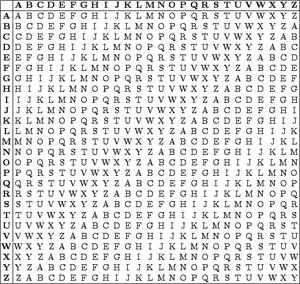
\includegraphics[width=0.6\columnwidth]{rkey.jpeg}
%	\caption{Tabula recta substitution function used to compute the ciphertext c letter-by-letter where c = (p + r) mod 26, where p is the plaintext and r is the running key.}	
%\end{figure}

\section{References}
Bauer, C. and Tate, C. (2002). A statistical attack
on the running key cipher. \textit{Cryptologia Volume 26, Issue 4}.\\
Griffing, A. (2006). Solving the Running Key Cipher with the Viterbi Algorithm. \textit{Cryptologia Volume 30, Issue 4}, pages 361-367.\\
Knight, K. and Reddy, S. (2012). Decoding Running Key Ciphers. \textit{Proceedings of the 50th Annual Meeting of the Association for Computational Linguistics},  pages 80-84.\\
\end{document}